\subsection{Rollator}
\noindent The most clear option for the choice of walker frame, to be outfitted with motors and the electronics system, is a standard medical rollator, available on common online commercial marketplaces. The model of choice is the Medline Premium Empower Rollator. The steel frame remains at a weight under 20 pounds, and its dimensions are given as 23.8"D x 11"W x 22"H. It comes with a seat, storage compartment, and pneumatically actuated brakes. The FORWARD team plans to remove the seat and storage compartment to replace with the electronics housing, change the braking system to velocity control, and to dismount the wheels to install the DC motors. The wheels are also 8 inch diameter, which we anticipate will provide enough torque for the adaptive velocity control and steering enacted by the motor shield.\\

\begin{figure}[H]
	\centering
	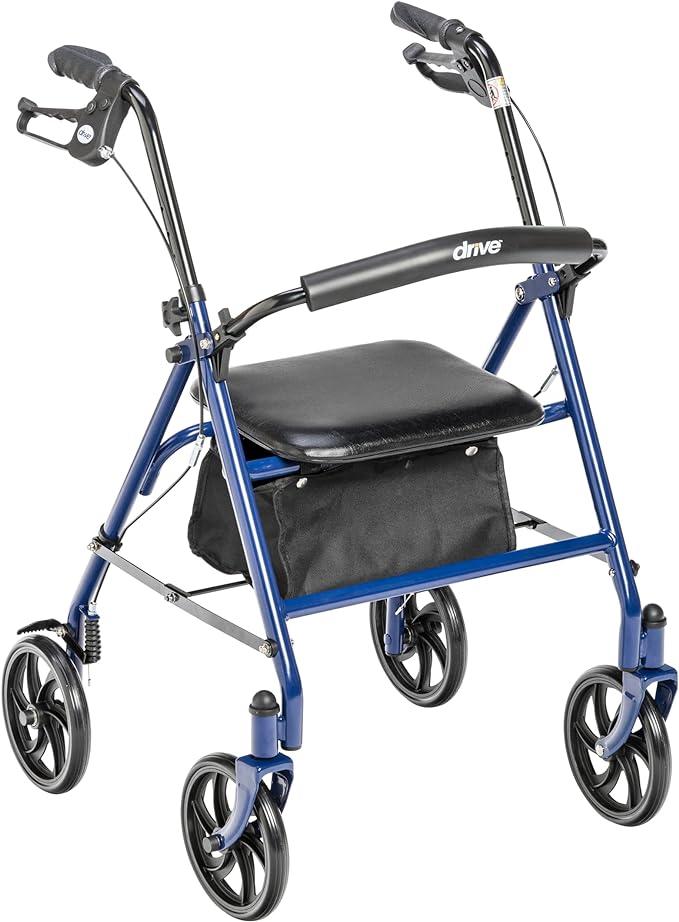
\includegraphics[width=0.3\textwidth]{./Images/rollator-amaz.jpg}
	\caption{\label{fig:rollator-amaz}Medline Premium Empower Medical Rollator}
\end{figure}

\noindent There are many other variants of rollators available - some with enlarged front wheels and some with only three wheels altogether. There seem to be two main shapes of frame: A and what we can call $\lambda$. We estimate that, the A frame is more appropriate for our purposes. FORWARD velocity control and electric braking also requires four wheels.\\

% morgan - do we fix the wheels in place? most of them swivel like castors

% matthew
\subsection{Electronics Chassis} \label{chassis}
% Discuss psychical location of all elements and components on the walker frame and explain the reason. explain plans for wiring and attachment (tape, glue, screws etc).
\subsubsection{Location of Components}
\noindent The diagram below depicts the physical location of the components as attached to the walker. Several components, including the power supply, Bluetooth module, PCB, IMU, and LiDAR will be housed within a hard casing, most likely made of metal or wood. They will be encased so that they are stable and not exposed to the elements. The LiDAR and IMU, both of which are mounted to the PCB, should not be allowed to change position. In particular, the IMU measures the angle of the walker and needs to be level. If the IMU is not level, it will give incorrect readings. It is also undesirable for the PCB to be unstable or mounted loose beneath the seat because it would be easy for connections to loosen or for vibration to damage sensitive parts. We will use screws to mount the internal components to this casing so that all of the units are fixed in place. All of the other components will need to have wires running to this casing. These wires will be organized and mounted against the walker using wire clips so that there are no dangling wires, which could be a tripping hazard to the user and would appear unprofessional.\\

\noindent For the components installed apart from the electronics case, we will use different methods of mounting depending on the nature of the component. The haptic motors will be located underneath the handlebars so that the user's hands are able to clearly sense the pattern of vibration. Each motor will be attached using a mounting bracket. This bracket will need to use tension or compression in order to secure the motors in place as the motors do not come with holes to mount to the back of the seat with screws. The headlight will be mounted on top of the backing of the walker seat. This location was chosen because it is the highest point of mounting for which the light can shine unobstructedly. It comes with a mounting bracket that will need to be attached to the walker using screws. The photoresistor may be attached to the headlight, out of the way of shadows, using a clip. There are four ultrasonic sensors that we will mount to the legs of the walker. Two will appear facing the front of the walker and the other two will appear on the side, angled toward front. The ultrasonic sensors contain small holes at each corner for mounting, however, it would be difficult to drill into the metal structure of the walker. We could use fishing rod clips to attach to the walker and mount the sensors to the clips.\\

\noindent The most difficult components to mount will likely be the DC motors driving the wheels. We must attach the motors in such a way that the wheel rotates as the rotor attached to the gearbox rotates. We also must ensure that the manual braking system is not eradicated, which limits our options to not mount the motor directly above the wheels. For example, we could detach the wheels from the hub and attach them directly to the motors whereas the motors are mounted to the walker. However, this would remove the braking mechanism from the wheels. Thus, we will mount the motor (using a connector piece screwed into the gearbox and the rim of the wheel) to the outside of the wheel and simply use a custom metal bracket to attach the motor to the leg of the walker. We will mount the two motors to the two rear wheels of the walker, as they are fixed, while the front two wheels swivel.\\ 

\begin{figure}[H]
	\centering
	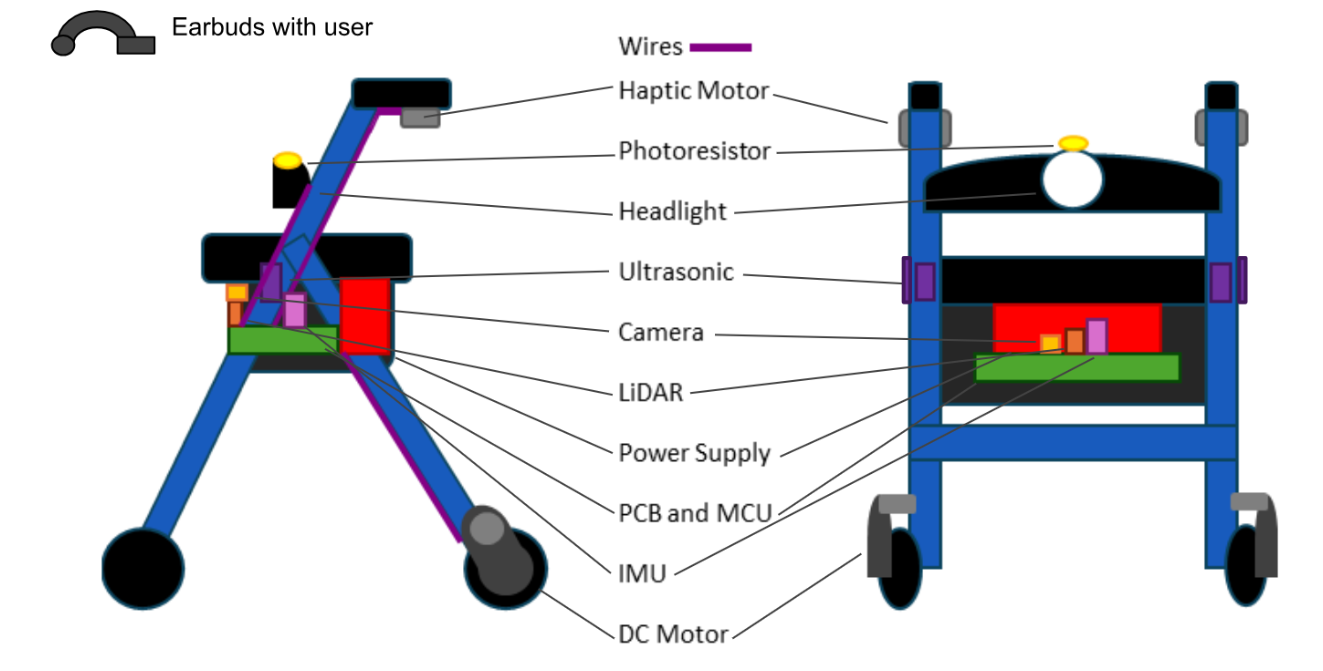
\includegraphics[width=1\textwidth]{./Images/component_location_ear.png}
	\caption{\label{fig:Component-Locations}Location of components on the walker}
\end{figure}

\subsubsection{Measurements of the Walker}
\noindent Upon purchasing the rollator chassis, we took measurements in order to design the placement of components on the walker. This is especially essential for obtaining the correct length of wires. We would like to have organized wires flush against the walker running from the PCB to different components, which requires precise measurements of the length of wires to appear professional. For example, we measured the distance from the wheel to the seat of the walker and will need to later add the measurement from the seat to the PCB housing underneath the seat. For Senior Design II, we will need the measurements for the PCB before we can start ordering the correct length of wires.\\

\begin{figure}[H]
	\centering
	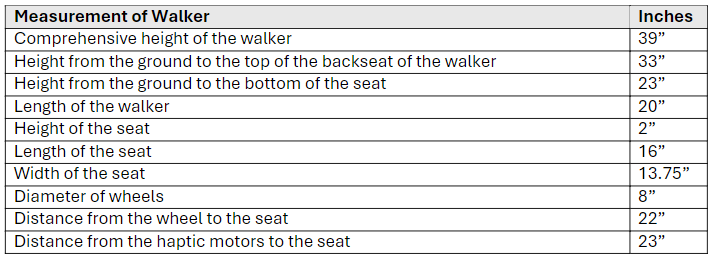
\includegraphics[width=1\textwidth]{./Images/measurements.png}
	\caption{\label{fig:Measurements_of_walker}Measurements of the walker}
\end{figure}

\noindent implementation of earpiece being available to user. physical object avoidance margins. obstacle classifications.\\

\noindent headlights? curb assist? tipover prevention with motors explained\\